%%%%%%%%%%%%%%%%%%%%%%%%%%%%%%%%%%%%%%%%%%%%%%%%%%%%%%%%%%%%%%%%%%%%%%%%%%%%%%%%
%%
%%   BornAgain User Manual
%%
%%   homepage:   http://www.bornagainproject.org
%%
%%   copyright:  Forschungszentrum Jülich GmbH 2015
%%
%%   license:    Creative Commons CC-BY-SA
%%
%%   authors:    Scientific Computing Group at MLZ Garching
%%               C. Durniak, M. Ganeva, G. Pospelov, W. Van Herck, J. Wuttke
%%
%%%%%%%%%%%%%%%%%%%%%%%%%%%%%%%%%%%%%%%%%%%%%%%%%%%%%%%%%%%%%%%%%%%%%%%%%%%%%%%%

\chapter{Instrument simulation}  \label{SInstr}

%%%%%%%%%%%%%%%%%%%%%%%%%%%%%%%%%%%%%%%%%%%%%%%%%%%%%%%%%%%%%%%%%%%%%%%%%%%%%%%%
\section{Detector images [TO REVISE]}\label{SdetImg}
%%%%%%%%%%%%%%%%%%%%%%%%%%%%%%%%%%%%%%%%%%%%%%%%%%%%%%%%%%%%%%%%%%%%%%%%%%%%%%%%

\def\tc{\text{c}}

%-------------------------------------------------------------------------------
\begin{figure}[t]
\begin{center}
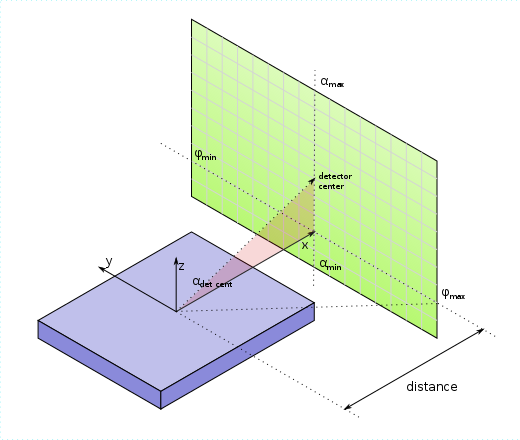
\includegraphics[width=.5\textwidth]{fig/drawing/experimental_geometry.png}
\end{center}
\caption{Experimental geometry with a two-dimensional pixel detector.}
\label{FexpGeom}
\end{figure}
%-------------------------------------------------------------------------------

To conclude this chapter on the foundations of small-angle scattering,
we shall derive the geometric factors
that allow us to convert differential cross sections into detector counts.
We shall also discuss how to present data on a physically meaningful scale.

%===============================================================================
\subsection{Pixel coordinates, scattering angles, and $\symbf{q}$ components}
%===============================================================================

We assume that scattered radiation is detected in a flat,
two-dimensional detector
that generates histograms on a rectangular grid,
consisting of $n\cdot m$ pixels of constant width and height,
as sketched in \cref{FexpGeom}.
This figure also shows the coordinate system
\index{Conventions|see {Coordinate system}}%
\index{Coordinate system}%
according to unanimous GISAS convention,
with $z$ normal to the sample plane,
and with the incident beam in the $xz$ plane.
The origin is at the center of the sample surface.
We suppose that the detector is mounted perpendicular to the $x$ axis
at a distance $L$ from the sample position.
%the $x$ axis intersects the detector plane at $(L,y_\tc,z_\tc)$.
The real-space coordinate at the center of pixel $(i,j)$ is $(L,y_i,z_i)$.
Each pixel has a width~$\Delta y$ and a height~$\Delta z$.
\index{Detector!pixel coordinate}%
\index{Pixel|see {Detector}}%

The affine-linear conversion from pixel indices $i,j$ to pixel coordinates $x_i,y_i$
requires an experimental calibration of the origin.
\Work{How is this done in \BornAgain?}
\index{Detector!calibration}%

Since the differential scattering cross section \cref{Exsectiondef}
is given with respect to a solid-angle element $\d\Omega$,
we need to express the scattered wavevector $\k_\tf$ in spherical coordinates,
using the horizontal azimuth angle~$\phi_\tf$
and the vertical glancing angle $\alpha_\tf$.
The projection of $(\alpha_\tf,\phi_\tf)$ into
the detector plane~$(y,z)$ is known as the \E{gnomonic projection}.
\index{Gnomonic projection}%
\index{Projection!wave vector to pixel coordinate}%
\index{Mapping!wave vector to pixel coordinate}%
\index{Transformation!wave vector to pixel coordinate}%
From elementary trigonometry one finds
\begin{equation}\label{Eyzdet}
  \begin{array}{lcl}
  y &=& L \tan\phi_\tf,\\
  z &=& (L/ \cos\phi_\tf) \tan\alpha_\tf.
  \end{array}
\end{equation}
\cref{Fconstalphi} shows lines of equal $\alpha_\tf$,~$\phi_\tf$
in the detector plane.
To emphasize the curvature of the constant-$\alpha_\tf$ lines,
scattering angles up to more than 25$^\circ$ are shown.
In typical SAS or GISAS,
scattering angles are much smaller,
and therefore the mapping between pixel coordinates and
scattering angles is in a good first approximation linear.
Of course \BornAgain\ is not restricted to this linear regime,
but uses the exact nonlinear mapping~\cref{Eyzdet}.

%-------------------------------------------------------------------------------
\begin{figure}[t]
\begin{center}
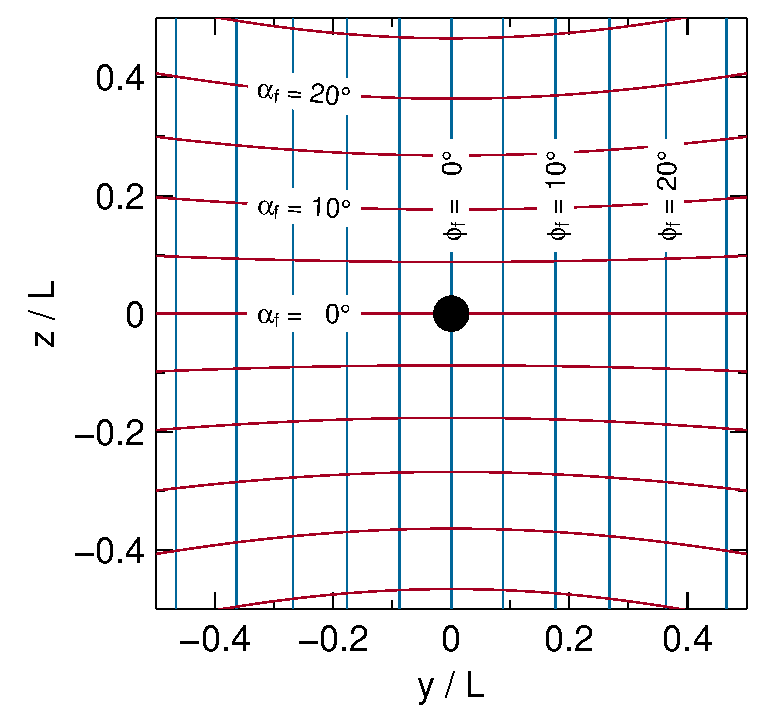
\includegraphics[width=.47\textwidth]{fig/drawing/SAS_const_alphi.ps}
\end{center}
\caption{Lines of constant $\alpha_\tf$ (red) or $\phi_\tf$ (blue)
in the detector plane,
for a planar detector at distance~$L$ from the sample.
The black dot indicates the beamstop location for
the central incident beam (SAS geometry, $\hat\k_\ti = \hat x$).}
\label{Fconstalphi}
\end{figure}
%-------------------------------------------------------------------------------

To determine the scattering vector $\q_{ij}$
that corresponds to a pixel $(i,j)$,
we need to express the outgoing wavevector~$\k_\tf$ as function of $y$ and~$z$.
This can be done either by inverting \cref{Eyzdet}
and inserting the so obtained $\alpha_\tf(y,z)$ and $\phi_\tf(y)$ in
\begin{equation}\label{Ekf_by_angle}
  \k_\tf=K\left(\begin{array}{c}
   \cos\alpha_\tf\cos\phi_\tf\\
   \cos\alpha_\tf\sin\phi_\tf\\
   \sin\alpha_\tf\end{array}\right),
\end{equation}
or much more directly by using geometric similarity in Cartesian coordinates.
The result is rather simple:
\Emph{
\begin{equation}\label{Ekf_by_pixel}
  \k_\tf=\frac{K}{\sqrt{L^2+y^2+z^2}}\left(\begin{array}{c}
   L\\
   y\\
   z\end{array}\right).
\end{equation}
\vspace*{-5pt}}


%-------------------------------------------------------------------------------
\begin{figure}[t]
\begin{center}
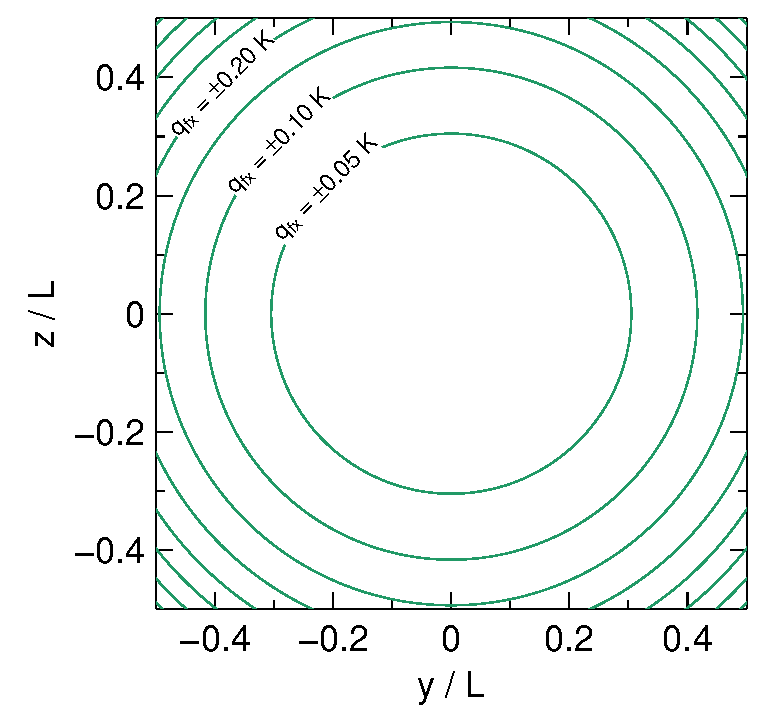
\includegraphics[width=.47\textwidth]{fig/drawing/SAS_const_q_x.ps}
\hfill
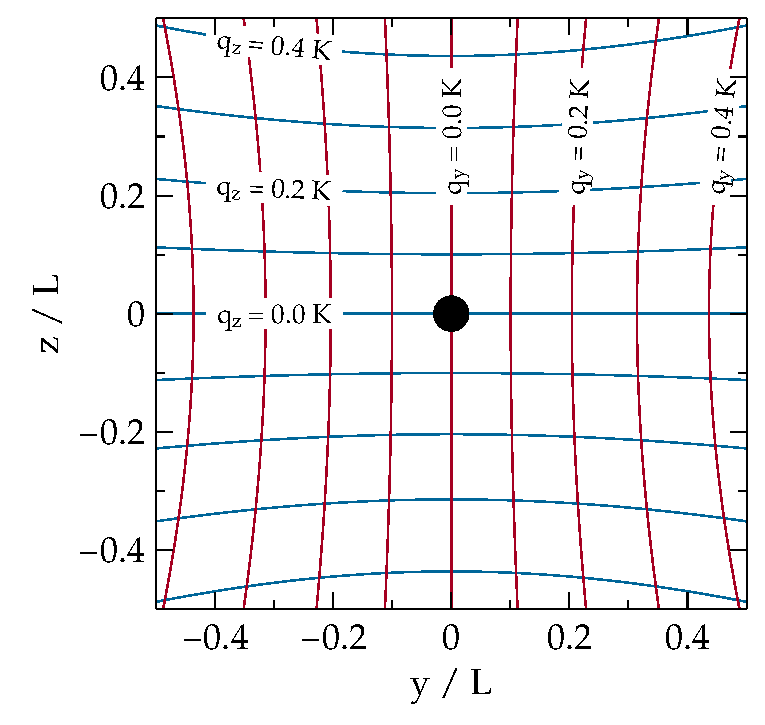
\includegraphics[width=.47\textwidth]{fig/drawing/SAS_const_q_yz.ps}
\end{center}
\caption{Lines of constant $q_x$ (left), $q_y$ or $q_z$ (right),
in units of the incident wavenumber $K=2\pi/\lambda$,
for a planar detector.
SAS geometry as in Fig.~\protect\ref{Fconstalphi}.}
\label{Fconstq}
\end{figure}
%-------------------------------------------------------------------------------

The transform \cref{Eqalgo} between pixel coordinates $y$,~$z$
and physical scattering vector components $q_y$, $q_z$
is nonlinear, due to the square-root term in the denominator of~\cref{Ekf_by_pixel}.
For $y,z\ll L$, however, nonlinear terms loose importance.

%-------------------------------------------------------------------------------
\begin{figure}[t]
\begin{center}
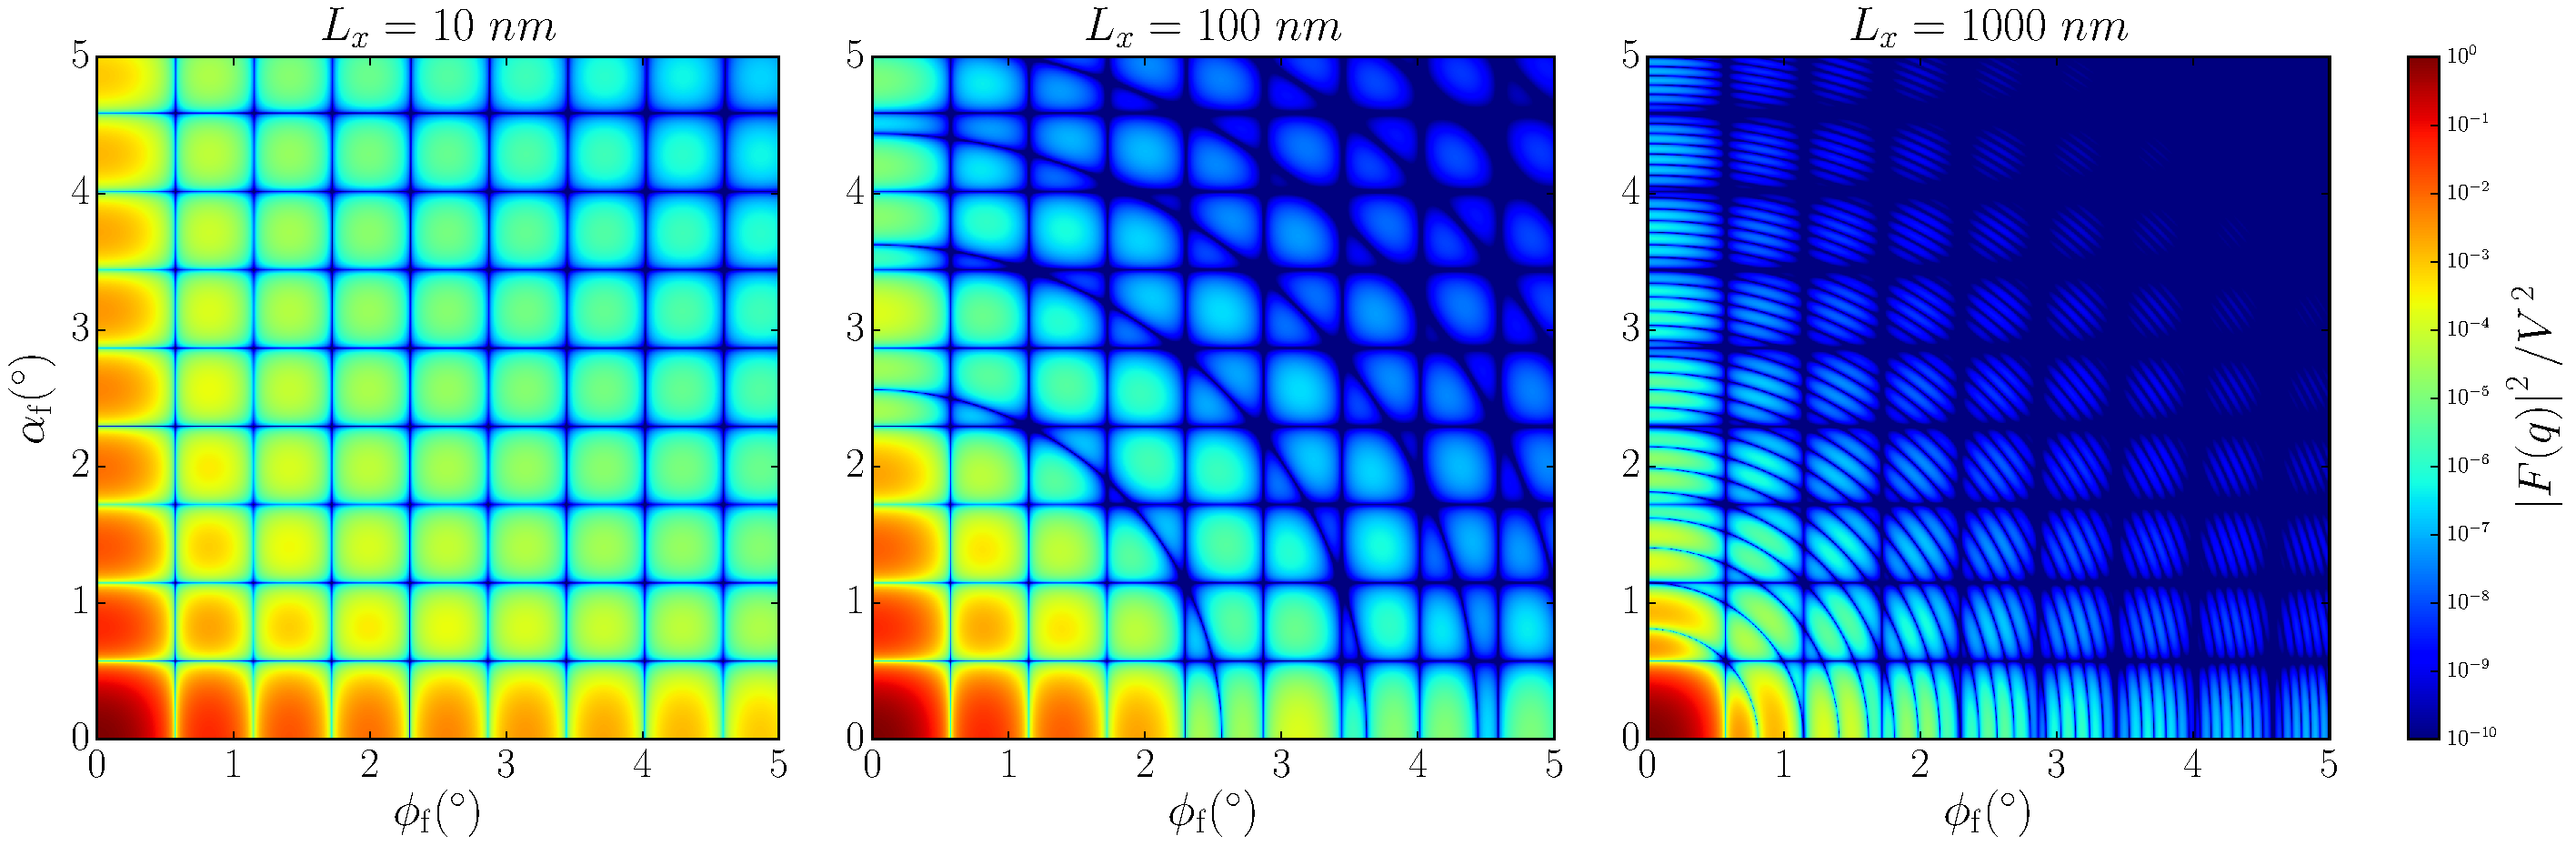
\includegraphics[width=1\textwidth]{fig/ff2/ff_det_box.pdf}
\end{center}
\caption{Simulated detector image for small-angle scattering from
uncorrelated cuboids (right rectangular prisms).
  \index{Box (form factor)}
  \index{Cuboid (form factor)}
  \index{Prism (form factor)!reactangular (Box)}
  \index{FormFactorBox@\Code{FormFactorBox}}
The incoming wavelength is 0.1~nm.
The prisms have edge lengths $L_y=L_z=10$~nm;
the length $L_x$, in beam direction, is varied as shown above the plots.
\index{Circular modulation!of detector image as function of $q_x$}
The circular modulation comes from a factor $\sinc(q_x L_x/2)$
in the cuboid form factor, with $q_x$ given by~\cref{Eqxasy}.}
\label{Fdetbox}
\end{figure}
%-------------------------------------------------------------------------------

The left detector frame in \cref{Fconstq}
shows circles of constant values of $\pm q_x$.
For given steps in $q_x$, the distance between adjacent circles
increases towards the detector center.
From \cref{Eq} and \cref{Ekf_by_pixel},
one finds asymptotically for $y,z\to L$
that $q_x$ goes with the square of the two other components of the scattering vector,
\begin{equation}\label{Eqxasy}
  \frac{q_x}{K}
  \doteq \frac{y^2+z^2}{2 L^2}
  \doteq \frac{q_y^2 + q_z^2}{2K^2}.
\end{equation}
Therefore, under typical small angle conditions $y,z\to L$
the dependence of the scattering signal on $q_x$ is unimportant:
one basically measures $v(\q)\simeq v(0,q_y,q_z)$.
The exception, for sample structures with long correlations in $x$~direction,
is illustrated in~\cref{Fdetbox}.

%-------------------------------------------------------------------------------
\begin{figure}[t]
\begin{center}
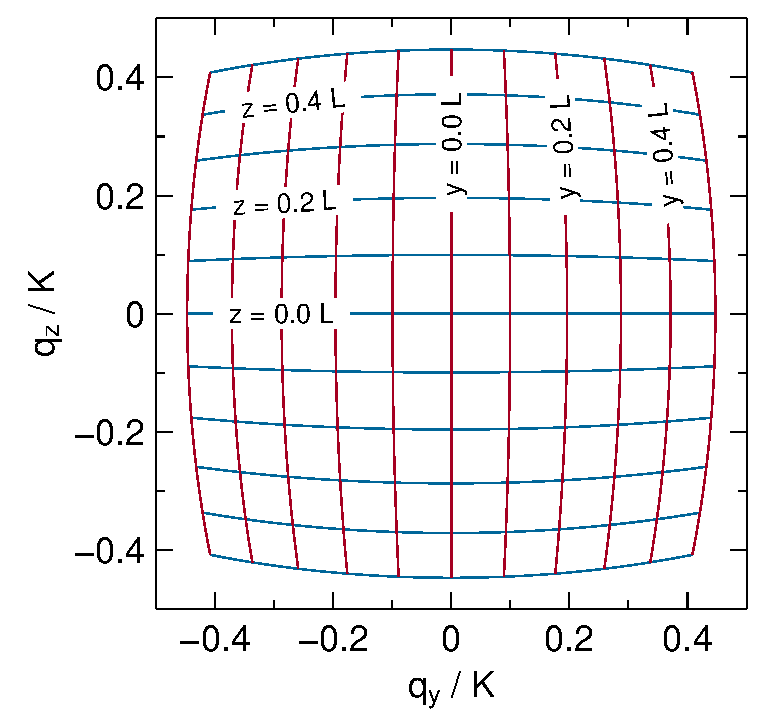
\includegraphics[width=.47\textwidth]{fig/drawing/SAS_const_p_yz.ps}
\end{center}
\caption{The outer contour of the blue and red grid
shows the border of a square detector image
after transformation into the physical coordinates $q_y$,~$q_z$.
The blue and red curves correspond to horizontal and vertical lines in the detector.}
\label{Fconstp}
\end{figure}
%-------------------------------------------------------------------------------

As anticipated in \cref{Eqxasy},
the other two components of $\q$ are in first order linear in the pixel coordinates,
\begin{equation}
  \frac{q_y}{K}=\frac{y}{L}\left(1-\frac{y^2+z^2}{2L^2}+\ldots\right),
\end{equation}
and similarly for~$q_z$.
The nonlinear correction terms lead to the pincushion distortion
shown in the right detector frame in \cref{Fconstq}.
\index{Distortion!of $q_x$, $q_y$ grid in detector plane}%
\index{Detector!distortion of $q_x$, $q_y$ grid}%
\index{Pincushion distortion}%

Since pixel coordinates are meaningful only
with respect to a specific experimental setup,
users may wish to transform detector images
towards the physical coordinates $q_y$ and~$q_z$.
As shown in \cref{Fconstp},
this would yield a barrel-shaped illuminated area
in the $q_y$,~$q_z$~plane.

To summarize this section,
the wavevector $\q_{ij}$ can be determined from the pixel indices
through the following steps:
\begin{equation}\label{Eqalgo}
  \begin{array}{cl}
      (i,j)&\\
      \downarrow&\mbox{calibrate of origin, then employ affine-linear mapping}\\
      (y,z)\\
      \downarrow&\mbox{use (\protect\ref{Ekf_by_pixel})}\\
      \k_\tf&\\
      \downarrow&\mbox{use (\protect\ref{Eq})}\\
      \q&\\
  \end{array}
\end{equation}

\Note{\indent Transforming detector images
  from pixel coordinates into the $q_y$,~$q_z$~plane is not implemented in \BornAgain,
  and not on our agenda.
  We would, however, like to hear about use cases.}

\Emph{\indent When simulating and fitting experimental data with \BornAgain,
detector images remain unchanged.
All work is done in terms of reduced pixel coordinates $y/L$ and~$z/L$.
Corrections are applied to the simulated, not to the measured data.}

\Work{\indent \ldots show how to plot $q$ grid on top of detector image \ldots}

%===============================================================================
\subsection{Intensity transformation}
%===============================================================================

The solid angle under which a detector pixel
is illuminated from the sample is in linear approximation
\begin{equation}
  \Delta\Omega
  = \cos\alpha_\tf\:\Delta\alpha_\tf\,\Delta\phi_\tf
  = \cos\alpha_\tf
    \left|\frac{\partial(\alpha_\tf,\phi_\tf)}{\partial(y,z)}\right|
    \Delta y \,\Delta z
  = \cos^3\!\alpha_\tf\, \cos^3\!\phi_\tf\: \frac{\Delta y \,\Delta z}{L^2}.
\end{equation}
\index{Detector!illumination angle correction factor}%
\index{Illumination!detector}%
Altogether,
the expected count rate in detector pixel $(i,j)$ is proportional to
\begin{equation}\label{EItrafo_cos}
  I_{ij} = \cos^3\!\alpha_\tf\, \cos^3\!\phi_\tf\:
          \frac{\partial\sigma}{\partial\Omega}(\q_{ij}),
\end{equation}
where we have omitted constant factors $L^{-2}$, $\Delta y$ and $\Delta z$.
Using pixel coordinates instead of angles, this can be rewritten as
\Emph{%
\begin{equation}\label{EItrafo_pix}
  I_{ij} = \left( 1+\frac{y^2+z^2}{L^2}\right)^{-3/2}
          \frac{\partial\sigma}{\partial\Omega}\bigl(\q_{ij}(y,z)\bigr).
\end{equation}
\vspace*{-2pt}}
%(usually as the centre between the transmitted
%and the specularly reflected beam spot).

%Tradition wants that raw data be \E{treated} or \E{reduced}
%before they are \E{analyzed}.
%In our case, raw data reduction would comprise
%the transform \cref{Eqalgo} of pixel coordinates into scattering vectors,
%and the accompanying renormalization \cref{EItrafo} of pixel counts.
